% In Latex the % symbol will indicate a comment. Text following the % symbol will not appear in the generated document and allow you to annotate your latex file
% This document is a modified version of the "sample document" provided by the American Journal of Physics through their author's guide.

\documentclass[prl,onecolumn]{revtex4-1}  % The "prl" tells latex to use the physical review letters formatting with one column from the revtex4.1 document class
%\documentclass[prl,preprint,linenumbers]{revtex4-1}  % other options can change formatting for various purposes. For example you can include line numbers with "linenumbers" and the "preprint" to make things easier to edit. Similarly you could use "singlecolumn" and "doublespace"
% NOTE: only a single documentclass should be declared. Comment out the other one. You can try changing styles and classes and compiling the document to see one of the benefits of Latex, the ease of reformatting.
\usepackage{physics}
\usepackage{mathrsfs}


% Latex has several packages that maybe needed to use things like figures or tables or certain math fonts. google is your friend. If there is something you want to do using latex, odds are several other people have wanted to do this in the past and a search for "how do you 'thing i want to do' in Latex" will likely lead to several forums and answers to your question.
\usepackage{amsmath}  % needed for \tfrac, \bmatrix, etc.
\usepackage{amsfonts} % needed for bold Greek, Fraktur, and blackboard bold
\usepackage{graphicx} % needed for figures
\usepackage{hyperref} % needed for clickable links
\usepackage{lipsum} 
\newcommand{\term}[0]{Fall 2018}  %Another great feature of Latex is it allows you to define macros (google "newcommand in latex" for details). Here i've made it so anytime i write \term the document will put Fall 2018. I can modify this command in future semesters and avoid having to find every instance in the document I refer to the semester of the class.

\begin{document}

% Be sure to use the \title, \author, \affiliation, and \abstract macros
% to format your title page.  Don't use lower-level macros to  manually
% adjust the fonts and centering.

\title{Crystal Luminescence }
% In a long title you can use \\ to force a line break at a certain location.

\author{Andrew Gonzales}
\email{gonza363@cougars.csusm.edu} % optional
% If there were a second author at the same address, we would put another 
% \author{} statement here.  Don't combine multiple authors in a single
% \author statement.
% Please provide a full mailing address here.
\affiliation{Department of Physics, California State University San Marcos, San Marcos, CA 92096}

\author{Joshua Lucas}
\email{Lucas035@cougars.csusm.edu}
\affiliation{Department of Physics, California State University San Marcos, San Marcos, CA 92096}

% See the REVTeX documentation for more examples of author and affiliation lists.
% or google

\date{\today}

\begin{abstract}
The emission of light from solids has been studied since the beginning of the seventeenth century with some mentions as far back as 6th century BCE %first citation
for reasons ranging from religious to aesthetic to pratical. There are several forms of luminescence that are differentiated based on the source of energy. They all have the same result: spontaneous emission of light. Not to be confused with incandescence, which is the emission of light due to thermal radiation. This tends to occur at relatively high temperatures. Luminescence is unique because it does not involve heating the substance and is possible even at room temperature. All types of luminescence involve a photon being emitted from an electron as it returns to its relaxed state after having been excitred by an energy source. Some common types of luminescence are photoluminescence, chemiluminescence, and electroluminescence. 
\\Phosphorus (light bearer)  
\\optical properties
\\applications



\end{abstract}
% All papers should include an abstract. 

\maketitle % title page is now complete


%\section{Introduction} % Section titles are automatically converted to all-caps.
%
%\section{Electron Orbitals}
%To understand the optical properties of solids we first need to understand the dynamics of an atom's  energy level. 
%\subsection*{Electron Configuration.. Pauli Exclusion}
%We can model the atom as being a positively charged nucleus orbited by a negatively charged electron. As the the number of electrons increases   The Pauli exclusion principal states that no two electrons in an single atom can exsist in the exact same state.  
%\subsection*{Closed shell... very stable}
%The electrons fully occupy orbital... shell is considered closed... harder to jump to higher level which makes it very stable..  
%\subsection*{Ground state..}
%Lowest energy level... preferred state of atom... 
%\subsection*{Valence Electrons...}
%The valence electron is in a open shell, less energy to raise its energy level
%\subsection*{Excited state..Absorption.}
%The electron jumps to a higher orbit with a higher energy level
%absorbs energy from a source all or nothing (quantum energy)
%
%
%\subsection*{Emission and Spectra}
%The orbital can relax down to a lower state, when it does it emits a photon where the wavelength is related to the quantized energy released.
%\begin{equation}
%E = \hbar \omega
%\end{equation}




\section{Electron Orbitals and energy}
To understand the optical properties of solids we first need to understand the dynamics of an atom's energy level. Electrons surround the nucleus of an atom in what is known as the electron cloud. The electron cloud is a general and often informal way of noting the locations where an electron is likely to be found. The electron cloud can be broken down into different energy levels. Which are in turn further broken down into sublevels. The sublevels are comprised of orbitals.

\par
We can model the atom as being a positively charged nucleus orbited by a negatively charged electron. This is known as the Bohr model. An important factor in describing the orbit of the electron is The Pauli Exclusion Principle. The Pauli Exclusion Principal states that no two electrons in an single atom can have the same quantum numbers. An electron's quantum numbers describe its orbit around the nucleus. This sets limits on the locations of the electrons within each orbital, and by extension each energy level.

\par
Electrons tend to want to be in their lowest possible energy configuration. Their options are somewhat limited, however thanks to the Pauli Exclusion Principle. When an atom's electrons are in their lowest possible energy level, we refer to that as the atom's ground state. 

\par
Atoms always react to reach more stable configurations. Many of these reactions can be described by the Octet Rule which states that atoms tend to prefer to have eight electrons in their outermost energy level, called the valence shell.

\par %drawing of energy levels w/ incoming photon
Atoms are often bombarded with different particles and the energy from these particles can be absorbed. The absorbed energy can even come from chemical reactions. As we have already stated, different sources of energy are the differentiating factor among types of luminescence. The absorbed energy is transferred to an electron and it jumps to a higher energy level. The difference in energy levels that the electron travels between is equal to the energy absorbed. For example, an electron that absorbs 10 eV will go to an energy level that is 10 eV higher than where it started. This is essentially conservation of energy. Not all amounts of energy are eligible to be absorbed, however. Energy amounts that equal the gap that an electron would jump have the highest probability to be absorbed. Otherwise, they are scattered in different forms with some cases of them not interacting at all, as we willl discuss later in this paper. When scattered, particles generally keep their form and are redirected while chemical energy is often radiated as heat. Electrons that have jumped to a higher energy level are referred to as excited electrons and likewise the state they are in is referred to as the excited state. Because possible states are limited, some electrons may need different wavelengths to jump to a higher available energy level. For example, an electron at energy level 1 can't jump to energy level 2 if it is full. Therefore, for that electron to become excited, it would need to absorb the corresponding energy amount to jump directly to energy level 3. The actual numerical values of these energy states vary from atom to atom, therefore the possible energies that are absorbed vary as well. The photonic equivalent of these absorbable energy levels make up the absorption spectrum which is unique to every atom.


\par
Electrons prefer to be in their ground state, sometimes referred to as their relaxed state. Once an electron is excited by an energy source, it will try to return to its relaxed state as soon as possible. As we will see, "soon" is a timescale that can vary upon a number of factors. In the case of photoluminescence (luminescence due to the absorption of photons), this timescale is the difference between fluorescence and phosphorescence. The method by which electrons return to their ground state is known as emission. Emission is the release of a photon by an electron as it moves to a lower energy state. Due to conservation of energy, this photon will have an energy corresponding to the difference in energy levels traveled by the electron, similar to absorption. The energy of a photon is dependent upon its wavelength as shown by the equation

\begin{equation}
E = \hbar \omega
\end{equation}

Different wavelengths correspond to different colors of light but the emission of photons is not limited to the visible light spectrum as there are a variety of possible energies that an electron can emit. The different wavelengths create the emission spectrum, similar to the absorption spectrum. Now that we have an understanding of the atom and how it emits light, we can begin to look at the structures of solids and how the arrangement of different atoms contribute to this process of luminescence.


\section{Energy Bands}
When we incorporate our understanding of electron energy levels in to a larger system of atoms, such as in a crystal, the model becomes further complicated due to the interactions of the surrounding atoms. The atoms bound together share the orbitals between them and following the Pauli principal only two electron eigenstates can occupy each orbital. If the number of atoms expands to the size of a macroscopic solid then the number of electrons, and in turn, orbitals becomes enormous. As the number of orbitals increase the change in energy levels between orbitals narrows so that for a continous line of atoms the enrgy level resembles a band  \cite{Levitin}. Calculating the total electron energy states of the system is vastly simplified by assuming the electron desinty will be periodic over the crsytal's own reciprocal k-space\cite{Lou}. The tight binding chain, also know as a linear combination of atomic orbitals, models the crystal as a chain of nuclei where an electron is capable of hopping across the chain. Although some simplifications are made on the interatomic interactions the results comapare with empirical measurments \cite{Elsevier}  We can use quantum mechanics to represent the electrons as a wave and can use the periodicity of the lattice to create a modified plane wave that is the result of multiplying the wave function by the periodic potential. This modified electron plane wave is know as a Bloch wave and the electron can traverse the system bound by the periodic potential without scattering\cite{Elsevier}. 
We have the Schr\"odinger equation for a single electron in some potential,
$
-\frac{\hbar^2}{2m} \nabla^2 \Psi_r = \big (E-V_0 \big) \Psi_r  
$
As the electron travels the periodic potential acting on it is   $V(r) = V(r+R)$, where $R$ is the translation vector. We can rearrange the Hamiltonian for the energy of the electrons in the periodic system,
\begin{equation}
\mathscr{H}\Psi(r) = \bigg [ -\frac{\hbar^2}{2m} \nabla^2 + V(r) \bigg ] \Psi(r) + E\Psi(r)
\end{equation} 
The solution to the energy simplyfies in to a function of k-space, where t is called the hopping term which is determined byt the distance between orbitals\cite{Simon}.
\begin{equation}
E = \epsilon_0 -2t\cos(ka)
\end{equation}
\begin{figure}[!h]
\centering
\includegraphics[width = .50\linewidth]{TightBindingChain.eps}
\caption{ Plot of Energy for the tight binding chain, one eigenstate for each point k space.}
\end{figure}

\par The electrons then only have one eigenstate at every point in k-space located in the first Brillouin zone forming continuous bands of energy where their eigenstates overlap. 
When we now include electrons for each atom in a chain they each contribute their valence electrons to the band. The Coulomb force on the nuclei and electrons seperate their energy levels in to isolated and merged bands\cite{Kittel}.  A monovalent atom, one valence electron, can only donate a single electron to the band where there are two possible spins to each eigenstate\cite{Simon}. The total number of atoms divided by the possible  spins leaves the band half full. The level that the states are filled is the Fermi surface. A small electric field can cause the some of the electrons to occupy higher orbitals, making the solid conductive and essentially a metal, we often find monavalent atoms are metals\cite{Simon}.  If the atom is di-valent, two valence electrons, the band will be fully filled with no increased states to occupy. A small electric field will have no effect as the energy levels are all filled, meaning the solid does not have metallic bonding will not conduct a current\cite{Simon}. An atom with three valence electrons will contribute two valence electrons to the first band, filling it , and one to the half filled second band. The first band being filled causes it to be immobile unless energy large enough is imparted to it to raise it out of its energy level\cite{Chen}. It is also possible for some configurations to halve overlapping energy level where after contributing its electrons neither the first or second bands are filled leaving the two partially filled bands to have interactions. 
\par
As the number of orbitals increase there are some that have no possible eigenstates creating whats known as a forbidden region between energy levels \cite{Levitin}. The lower filled band is the valence band and the upper empty band is the conduction band. The distance of the gap between energy levels determines if a solid is a conductor, semi-conductor, or insulator. For the electrons to be excited to the higher band they must have the amount of between the gaps, band gap energy, imparted onto them. A low energy photon that is below the band gap energy  can not be absorbed by the solid, instead it passes through. If a photon is above the band gap energy then an electron can be excited up to the conduction band. This is what makes some materials transparency or the color of their appearance. If the energies of all wavelengths of visible light are below the band gap then the material is transparent where if only one frequency is below only that color of light is unabsorbed and passes through giveing the solid a hue\cite{Simon}. There is also the possibility of a energy transition to be made due to an indirect gap where the upper conduction band is closer at some point in k-space so the electron travels through k-space. For conservation of momentum an electron needs to travel in a direct transition from a lower band to upper band at the same point in k-space. During a indirect transition the momentum is also conserved by the production of a phonon inside the crystal. \cite{Simon} 
\par
When an electron makes a trasistion from the valence band to the conduction band it leaves behind whats called an electron hole and behaves as a positive charge in appiled electric and magnetic fields \cite{Kittel}. The density of electrons in the conduction band is referred to as n which is for negative charge, and the density of holes is called p for positive charge. The basis for the pnp and npn transistors comes from the energy band dynamics of solids.  
When a electron bridges the energy gap to the conduction band it and the hole left behind, which can also move through the crystal, effect the conductivity of the solid\cite{Chen}.


\section{Luminescence}
 
\subsection*{Tribolumincence..}
\subsection*{sonolumincence..}
\subsection*{cathode..}
\subsection*{scintillation..}

see through glass, crystals cant bridge gap..
Excite energy level, relax back and emit photon.. UV..
impurities...
Change color... hue
\subsection*{Defects...}
\subsection*{Traps...}
Pattern?...
Doping affects band gap...

\section{Applications}
Identification of material through emission lines.
\subsection*{Scintillation...}
particle detection.




\section{Endnotes and references}


\section{Conclusion}



\appendix*   % Omit the * if there's more than one appendix.

\section{Uninteresting stuff}



\begin{acknowledgments}

We gratefully acknowledge the American Journal of Physics for providing a sample
\LaTeX\ document that was easy for me to edit and adapt for this purpose. 

\end{acknowledgments}


\begin{thebibliography}{99}
% The numeral (here 99) in curly braces is nominally the number of entries in
% the bibliography. It's supposed to affect the amount of space around the
% numerical labels, so only the number of digits should matter--and even that
% seems to make no discernible difference.



\bibitem{Kittel} Kittel, C Introduction to Solid State Physics [233]

\bibitem{Virk} Virk, H. S. (Ed.). (2013). Luminescence related phenomena and their applications : special topic volume with invited peer reviewed papers only. 

\bibitem{Gotze} G\"otze J  Anal Bioanal Chem (2002) 374 :703–708

\bibitem{Lou}Lou, L. (2003). \textit{Introduction to phonons and electrons}[171].
\bibitem{Elsevier} Solid State Physics 2000, Elsevier Science \& Technology, London.[168, 171]
\bibitem{Chen} Chen, R., Pagonis, V., \& Lawless, J. L. (2010). \textit{Thermally and optically stimulated luminescence : a simulation approach. }[8]
\bibitem{Simon} Simon, S Oxford Solid State Basics [102, 104]

\bibitem{Levitin} Levitin, V 2013, Interatomic Bonding in Solids : Fundamentals, Simulation, Applications, John Wiley \& Sons, Incorporated, Weinheim. [79]

\end{thebibliography}




\end{document}
